\documentclass[t]{beamer} \usepackage[english]{babel} \usepackage[utf8]{inputenc} \usetheme{Frankfurt} %{{{
\usefonttheme{serif} \usepackage{palatino}
\let\OLDsection\section \renewcommand{\section}[1]{\OLDsection{#1} \subsection{}} % each slide has a bullet even when no subsections used
\usepackage{booktabs,amsmath,amsfonts,graphicx,sidecap}
\usepackage{tikz} \tikzstyle{every picture}+=[remember picture] \everymath{\displaystyle}
\usepackage{textpos} 

\beamersetleftmargin{3mm} \beamersetrightmargin{3mm}
\definecolor{myblue}{rgb}{0.10, 0.30, 0.50}
\usecolortheme[named=myblue]{structure}
\setbeamertemplate{navigation symbols}{\color{myblue}\footnotesize\insertframenumber}			% leave only tiny page number at the bottom
\setbeamerfont*{frametitle}{size=\normalsize,series=\bfseries}
%}}}
\hypersetup{
        pdftitle={Metamaterials for the Terahertz Spectral Range},
        pdfauthor={Ing. Filip Dominec},
        pdfsubject={},
        pdfkeywords={}
}

\usepackage[
  language=english,
  %urldate=long,
  style=numeric,
  sorting=none,
  isbn=true,
  doi=false,
  url=true,
  firstinits=true,  % will render all first and middle names as initials.
  abbreviate=false,
  autolang=hyphen,
  backend=biber,
  maxbibnames=3]{biblatex}
\renewbibmacro{in:}{%
  \ifentrytype{article}{}{\printtext{\bibstring{in}\intitlepunct}}}
% Volume number must be typeset in bold
\DeclareFieldFormat[article]{volume}{\textbf{#1}}% volume of a journal

% Pages must not be leaded by any "Pages:" word
\DeclareFieldFormat[article]{pages}{#1}% volume of a journal

% Year must be in paretheses
\DeclareFieldFormat[article]{date}{\mkbibparens{#1}}

% Remove quotation of title
\DeclareFieldFormat
  [article,inbook,incollection,inproceedings,patent,thesis,unpublished]
  {title}{#1\isdot}

% Comma NOT before BUT after journal volume
    \renewbibmacro*{volume+number+eid}{%
      %\setunit*{\addcomma\space}% NEW
      \printfield{volume}%
    %  \setunit*{\adddot}% DELETED
      %\setunit*{\addcomma\space}% NEW
      %\printfield{number}%
      %\setunit{\addcomma\space}%
      \printfield{eid}
}





% Comma before date; date not in parentheses
\renewbibmacro*{issue+date}{%
  %\setunit*{\addcomma\space}% 	 DELETED comma
%  \printtext[parens]{% DELETED
    \iffieldundef{issue}
      {\usebibmacro{date}}
      {\printfield{issue}%
       %\setunit*{\addspace}%
%       \usebibmacro{date}}}% DELETED
       \usebibmacro{date}}% NEW
  \newunit}

% Issue/date macros removed after journal number
\renewbibmacro*{journal+issuetitle}{%
  \usebibmacro{journal}%
  \setunit*{\addspace}%	 RETURNED HERE, avoid dot or comma after journal name
  \iffieldundef{series}
    {}
    {\newunit
     \printfield{series}%
     %\setunit{\addspace}}%	 DELETED comma
	}
  \usebibmacro{volume+number+eid}%
%  \setunit{\addspace}% DELETED
  %\usebibmacro{issue+date}% DELETED
%  \setunit{\addcolon\space}% DELETED
%  \usebibmacro{issue}% DELETED
  \newunit}

% "In:" removed for articles; issue/date macros added after note+pages macro
\DeclareBibliographyDriver{article}{%
  \usebibmacro{bibindex}%
  \usebibmacro{begentry}%
  \usebibmacro{author/translator+others}%
  \setunit{\labelnamepunct}\newblock
  \usebibmacro{title}%
  \newunit
  \printlist{language}%
  \newunit\newblock
  \usebibmacro{byauthor}%
  \newunit\newblock
  \usebibmacro{bytranslator+others}%
  \newunit\newblock
  \printfield{version}%
  \newunit\newblock
%  \usebibmacro{in:}% DELETED
  \usebibmacro{journal+issuetitle}%
  \newunit
  \usebibmacro{byeditor+others}%
  \newunit
  \usebibmacro{note+pages}%
  \usebibmacro{pageref}% MOVED HERE
  \setunit{\addspace}% NEW
  \usebibmacro{issue+date}% NEW
  \setunit{\addcolon\space}% NEW
  \usebibmacro{issue}% NEW
  \newunit\newblock
  \iftoggle{bbx:isbn}
    {\printfield{issn}}
    {}%
  \newunit\newblock
  \usebibmacro{doi+eprint+url}%
  \newunit\newblock
  \usebibmacro{addendum+pubstate}%
  \setunit{\bibpagerefpunct}\newblock
  %\usebibmacro{pageref}%
  \usebibmacro{finentry}}

\addbibresource{../fdphd.bib}



\title[THz MMs]{Metamaterials for the Terahertz Spectral Range\\ Ph. D. dissertation defence}
\author{Ing. Filip Dominec} 
\institute{Advisor: Dr. Mgr. Filip Kadlec (Fyzikální ústav AVČR)\\ Consultant: doc. Dr. Ing. Ivan Richter (FJFI ČVUT)\vspace{2mm}\\ Opponents: doc. Ing. Lukáš Jelínek, Ph.D.,\\
and doc. Dr. Mgr. Kamil Postava (VŠB-TU Ostrava) } 
\date{13$^{\mathrm{th}}$ December 2016}


\newcommand{\E}{\mathbf{E}}
\newcommand{\D}{\mathbf{\tilde{D}}}
\newcommand{\Dsd}{\mathbf{D}}
\newcommand{\B}{\mathbf{B}}
\newcommand{\HH}{\mathbf{\tilde{H}}}
\newcommand{\HHsd}{\mathbf{H}}
\newcommand{\epsrl}{\varepsilon_r}
\newcommand{\murl}{\mu_r}
%\newcommand{\epsrl}{\varepsilon^{\rm(Loc)}_r}
%\newcommand{\murl}{\mu^{\rm(Loc)}_r}
\newcommand{\Neff}{N_{\text{eff} }}
\newcommand{\Zeff}{Z_{\text{eff} }}
\newcommand{\eeff}{\varepsilon_{\text{eff} }}
\newcommand{\meff}{\mu_{\text{eff} }}
\newcommand{\ii}{{\mathrm i}}
\newcommand{\rr}{{\mathbf{r}}}
\newcommand{\brho}{\boldsymbol{\rho}}
\newcommand{\kk}{{\mathbf{k}}}
\newcommand{\KK}{{\mathbf{K}}}
\newcommand{\epsr}{{\varepsilon_r}}

\newcommand{\add}[1]{\color{blue}#1\color{black}{}}
\newcommand{\rmv}[1]{\color{grey}\ensuremath{\vdash}#1\ensuremath{\dashv}\color{black}{}}
\newcommand{\mdf}[1]{{\color{red}#1}}
\newcommand{\coloruse}{\marginpar{\scriptsize
\add%
{added}\\ \mdf%
{modified}\\ \rmv%
{deleted} }}



\begin{document}

\section{Introduction}
\begin{frame}		%{{{ Titulní stránka
	\titlepage
\end{frame}		%}}}
%\begin{frame}[plain]{\tiny{\vspace{-1em}A text\vspace{-.5em}}}	%{{{

%\begin{array}
%\nabla \cdot  \D = 0,\\
%\nabla \cdot  \B = 0,\\
%\nabla \times \E = -\frac{\partial \B} {\partial t},\\
%\nabla \times \HH =  \frac{\partial \D} {\partial t},
%\end{array}

\begin{frame}{What are metamaterials?} 		%{{{
Usually, metamaterials are periodic structures artificially designed to achieve some values of \textit{effective parameters} that are not found in natural materials.

\begin{exampleblock}{Proposed definition}
A metamaterial is any inhomogeneous structure that we attempt to describe as a homogeneous one
\end{exampleblock}

Then, the task of finding the effective parameters (homogenisation) is more fundamental than just a means of characterisation: It \textit{defines} that the structure \textit{is} a metamaterial.
\end{frame} 		%}}}

\begin{frame}[plain]{\tiny{\vspace{-1em}{Early metamaterials -- artificial dielectrics}\vspace{-.5em}}} 		%{{{
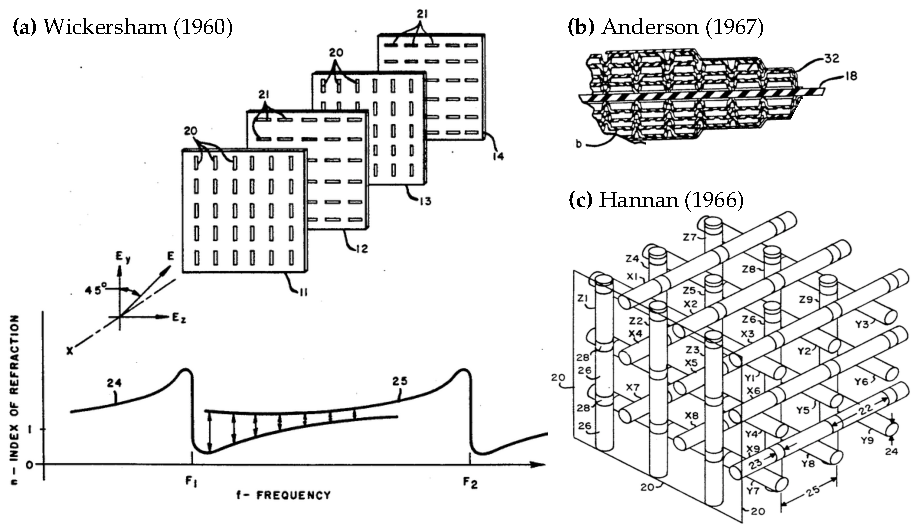
\includegraphics[width=\textwidth]{img/patents/mm_patents.pdf} 

%\textbf{(a)} sheets containing cut wires of alternating orientation and resonant frequency, enabling one to manipulate the microwave polarisation, \textbf{(b)} cross-section through a lightweight lens of 3 m diameter designed for 50-500 MHz radio waves, made of partially metallized plastic layers, \textbf{(c)} artificial dielectric made of non-resonant cut wires arranged into a nearly isotropic 3-D lattice. 
\vfill
\tiny{J. A. F. Wickersham. Artificial dielectric polarizer. US Patent 2,921,312. 1960. URL : http://www.google.com/patents/US2921312.\\
D. L. Anderson. Artificial dielectric lens structure. US Patent 3,329,958. 1967. URL : http://google.ru/patents/US3329958.\\
P. W. Hannan. Artificial dielectric using interspersed rods. US Patent 3,254,345. 1966. URL : http://www.google.com.py/patents/US3254345.}
\end{frame} 		%}}}


	\begin{frame}{Early photonic crystals} 		%{{{
PhCs are periodic structures aimed at engineering the photonic band gap and density of states. 
Their effective parameters are usually not determined.

Probably the first PhC, proposed by E. Yablonovitch in 1987, was manually drilled into a block of acrylic glass.

\vfill
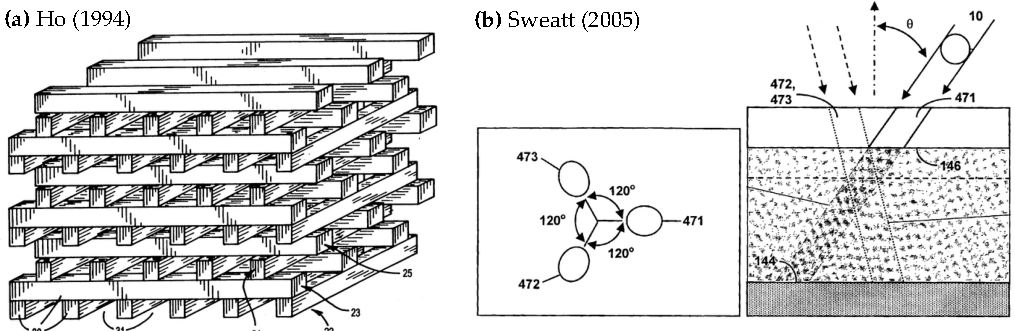
\includegraphics[width=\textwidth]{../img/patents/phc_patents.pdf} 
\vfill

\tiny{E. Yablonovitch. Inhibited Spontaneous Emission in Solid-State Physics and Electronics. Phys. Rev. Lett. 58, 2059–2062 20(1987).\\
K. Ho, C. Chan, and C. Soukoulis. Periodic dielectric structure for production of photonic band gap and devices incorporating the same. US Patent 5,335,240. 1994.  URL : https://www.google.com.ar/patents/US5335240.\\
W. Sweatt and T. Christenson. Method for the fabrication of three-dimensional microstructures by deep X-ray lithography. US Patent 6,875,544. 2005. URL : https://www.google.com.ar/patents/US6875544.  }
\end{frame} 		%}}}

\begin{frame}{2000's: Merging of MM and PhC paradigms?} 		%}}}
Two paradigms metamaterials (earlier denoted as artificial dielectrics) and photonic crystals developed separately over few decades.

They differed in the ratio of periodicity $a$ compared to the wavelength $\lambda$. 

\begin{exampleblock}{Waves in periodic structures vs. in natural media}
\centering \begin{tabular}{lcccr}
Light in MMs    &$\leftrightarrow$  &$\lambda \gg a$ &$\leftrightarrow$ 	& Light in a crystal         	\\
Light in PhCs   &$\leftrightarrow$  &$\lambda \sim a$ &$\leftrightarrow$ 	& Electron wave in a crystal 	\\
\end{tabular}
\end{exampleblock}

\end{frame} 		%}}}



\begin{frame}{2000's: Merging of MM and PhC paradigms?} 		%}}}
However, as the metamaterial research approaches the optical frequencies,  the $\lambda \gg a$ limit can not be held
Since 2000s, the research is getting into the boundary region between PhCs and MMs. [citations of NIR/optical MMs] 

Note that this is determined by available materials (not a mere issue of today's technology)

We must carefully review all approaches to MMs that assumed the unit cell $a$ to be \textit{just small}
\end{frame} 		%}}}


\section{Dielectric-rod array}

\begin{frame}{The structure under investigation}	%{{{

Dielectric-rod photonic crystal (with $\varepsilon_r$ = 100)  [TODO - citations]

Dielectric-rod metamaterial (with $\varepsilon_r$ = 100) [TODO - citations again]

\end{frame} 		%}}}

\begin{frame}{}	%{{{
PhC with r/a=0.1
\end{frame} 		%}}}

\begin{frame}{}	%{{{
negative-index MM r/a=0.12

\end{frame} 		%}}}

\begin{frame}{}	%{{{
Changing the radius-to-period parameter - continuous

\end{frame} 		%}}}

\begin{frame}{}	%{{{
Changing the radius-to-period parameter - user plot [cite our paper]

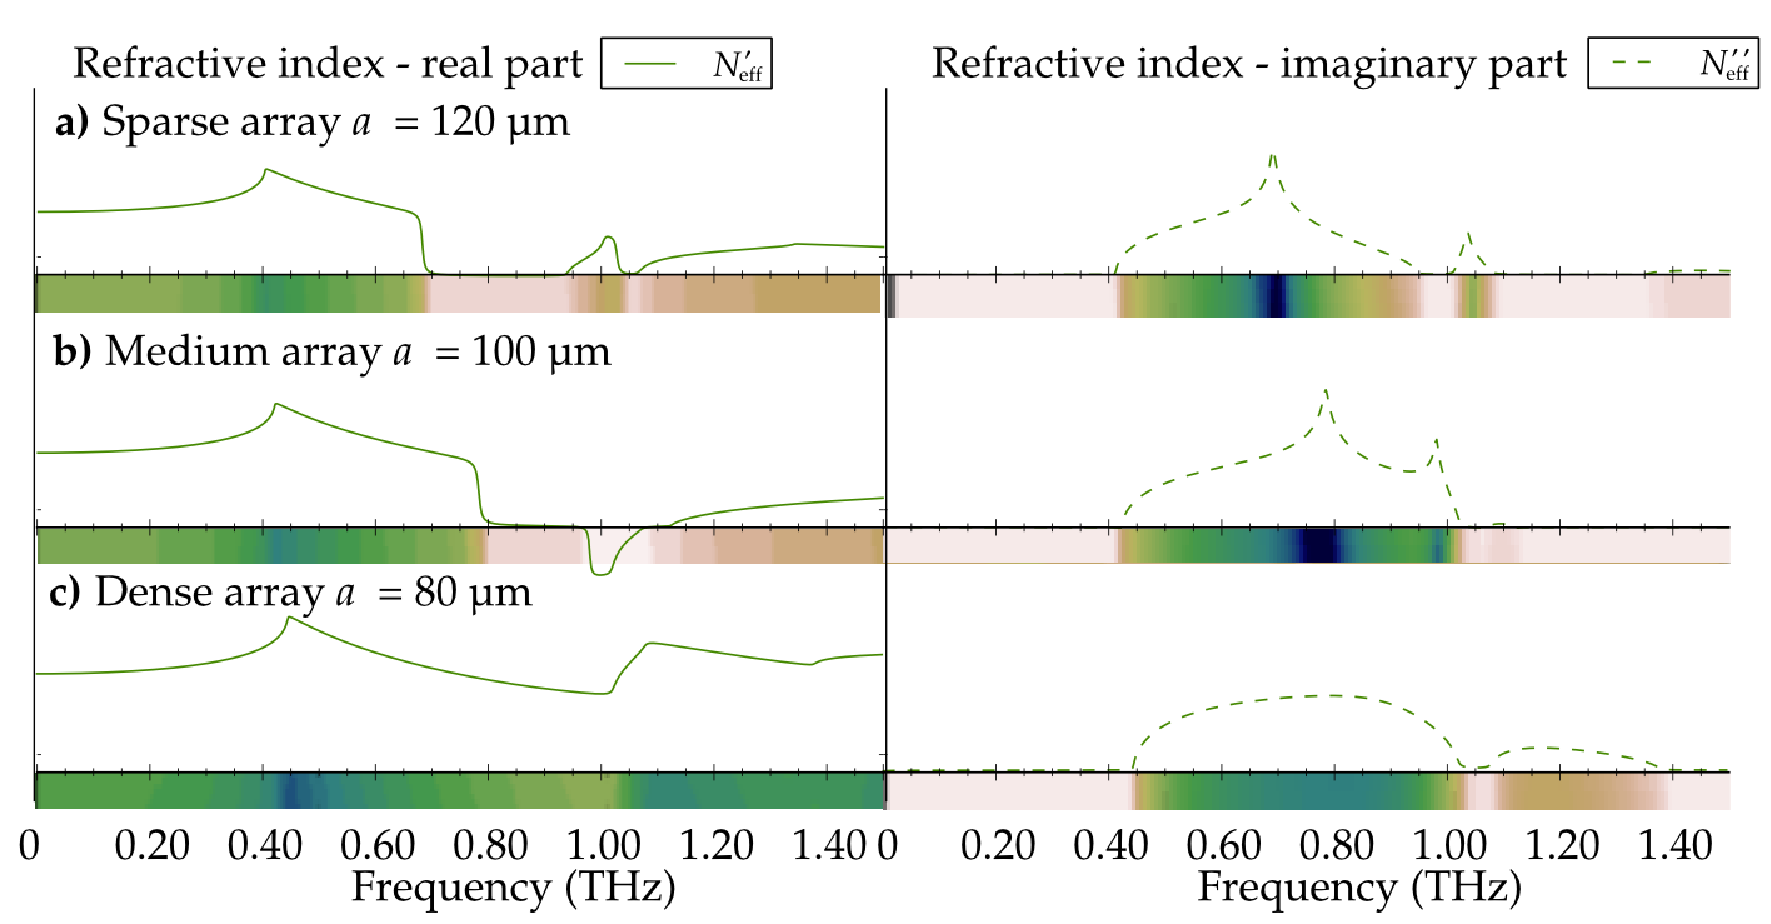
\includegraphics[width=1.\framewidth]{../img/ERods_sketch_of_separate_spectra_to_continuous_scan.pdf}

\end{frame} 		%}}}

\begin{frame}{}	%{{{
Do effective local $\eeff$ and $\meff$ make any sense? [TODO citations and screens from 'Antiresonance discussion']

We arrived to a metamaterial where N makes physical sense, but it makes no physical sense to transform N into effective $\eeff$ and $\meff$.
\end{frame} 		%}}}

\begin{frame}{}	%{{{
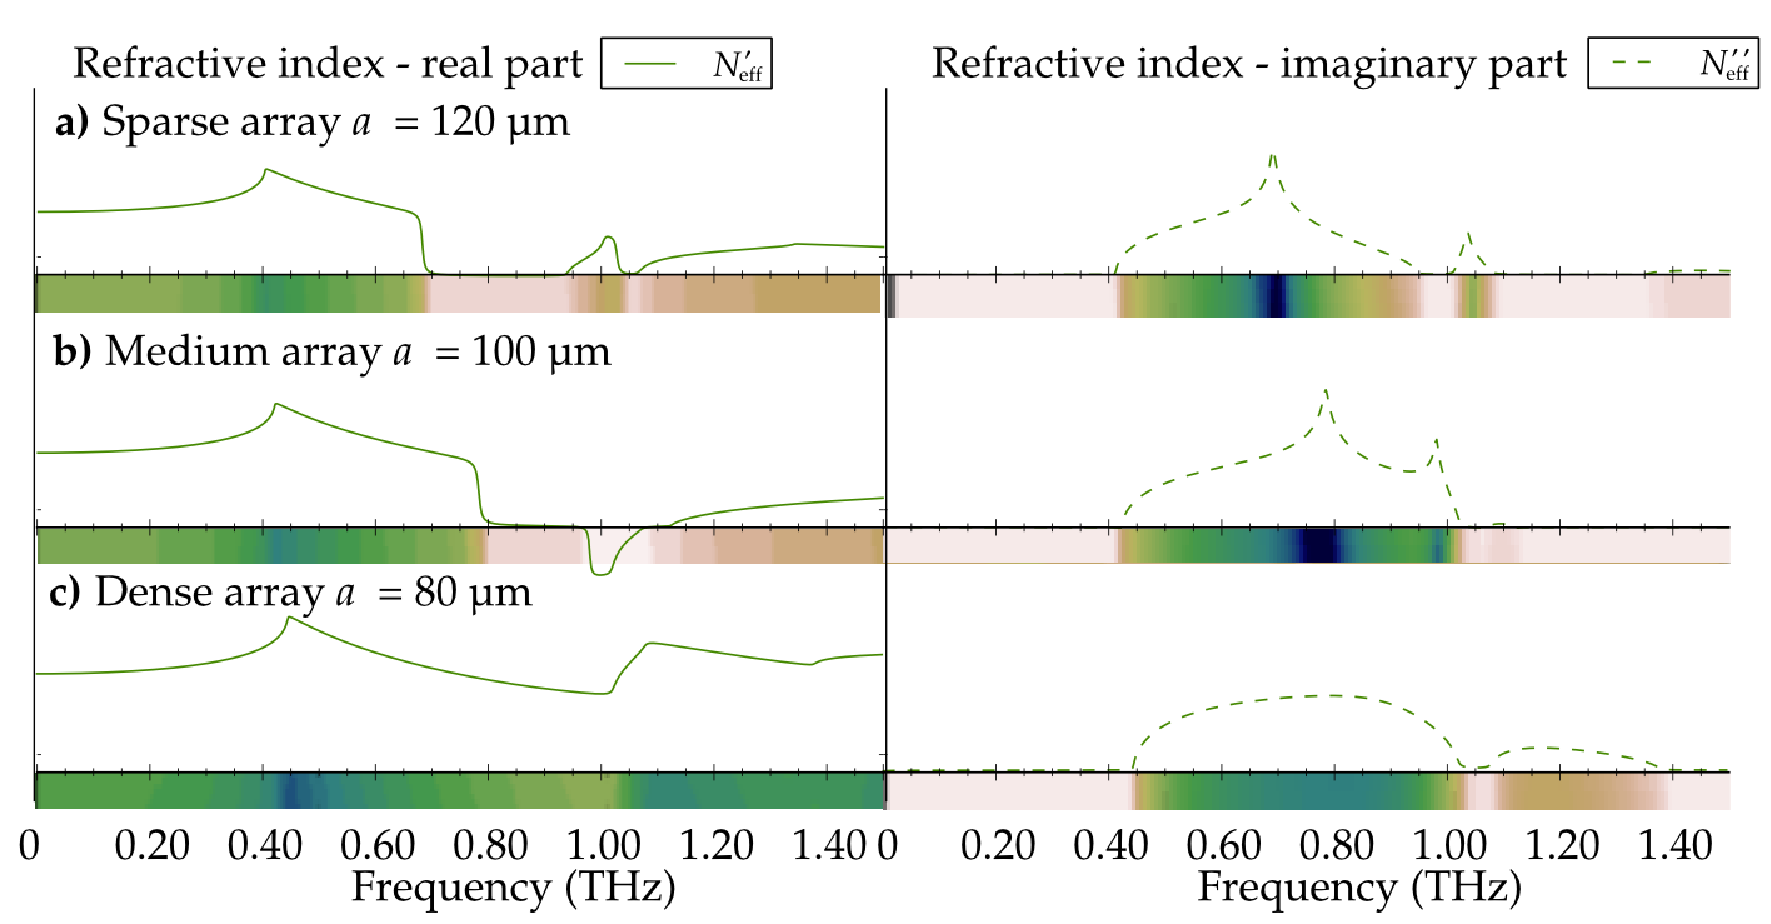
\includegraphics[width=1.\framewidth]{../img/ERods_sketch_of_separate_spectra_to_continuous_scan.pdf}
\end{frame} 		%}}}


\begin{frame}{The metamaterial assumption $\lambda_0 \gg a$ is unsustainable}	%{{{
	{\vspace{-.1em}\hfill \ldots for majority of realistic metamaterials}

\vspace{-1em}
\begin{table}[ht]   \caption{Short survey for the ratio of free-space wavelength $\lambda_0$ to the unit-cell size (parallel and perpendicular to $\kk$) in selected publications}  \label{tb_} \centering 
\begin{tabular}{lrrrr}
\toprule
	Source		 & $\lambda_0$ (nm)	& $\lambda_0/a_{||}$  & $\lambda_0/a_{\perp}$ & type \\
\hline
Šindler et al. 2016  & 350000		&  6--10	& 6--10 & Mie \\
Zhang et al. 2005    & 1300			&  7.5      & \textbf{2.2}  & SRR \\
Dolling et al. 2007  & 780			&  8		& \textbf{2.6}  & fishnet \\
Gong et al. 2014     & 565			&  8.0		& \textbf{2.4}  & fishnet \\
Aslam et al. 2012    & 510			&  14		& \textbf{2.1}  & fishnet \\
Xu et al. 2013	     & 365		    & \textbf{2.4}		& N/A	& 2-D layers \\
\bottomrule
\end{tabular} \end{table}

	\vfill
	\tiny{	
Šindler, M., et al. . Bulk magnetic terahertz metamaterials based on dielectric microspheres. Optics Express, 24(16), 18340-18345, (2016).\\
Zhang, S. et al.  Midinfrared resonant magnetic nanostructures exhibiting a negative permeability. Physical review letters, 94(3), 037402 (2005).\\
Dolling et al. Negative-index metamaterial at 780 nm wavelength. Opt. Lett. 32, 53–55 (2007)\\
Gong, B., et al.,. A visible metamaterial fabricated by self-assembly method. Scientific reports, 4 (2014).\\
Aslam, M. I., and Güney, D. Ö. . Dual-band, double-negative, polarization-independent metamaterial for the visible spectrum. JOSA B, 29(10), 2839-2847 (2012).\\
Xu, T., et al.. All-angle negative refraction and active flat lensing of ultraviolet light. Nature, 497(7450), 470-474  (2013).}
\end{frame} 		%}}}







\section{Nonlocal response}
\begin{frame}{Nonlocal response}%{{{
	The trouble with using $\eeff(\omega)$ and $\meff(\omega)$ is that they only describe the local response. \vspace{.5em}

The medium may be \textit{nonlocal}, i.e., elecric field in point $\rr$ makes it develop polarisation also in surrounding points $\rr\neq\rr'$.
	
\begin{exampleblock}{Waves in periodic structures vs. in natural media II.}
\centering \begin{tabular}{lcccr}
Light in MMs    &$\leftrightarrow$  &$\lambda \gg a$ &$\leftrightarrow$ 	& Light in a crystal         	\\
Light in PhCs   &$\leftrightarrow$  &$\lambda \sim a$ &$\leftrightarrow$ 	& Electron wave in a crystal 	\\
	\textbf{Previous example}  &$\leftrightarrow$  &$\mathbf{\pmb{\lambda\lesssim a}}$ &$\leftrightarrow$ 	& \textbf{Nonlocal medium!}\\
\end{tabular}
\end{exampleblock}

For a harmonic wave, nonlocality translates into \textit{spatial dispersion}, and the effective parameters explicitly depend on the wave vector $\kk$: 
$$\epsrn(\omega,\kk), \murn(\omega,\kk)$$
\end{frame} %}}}

\begin{frame}{Transforming $\epsrn(\omega,\kk), \murn(\omega,\kk)$ into the EBD form}%{{{
Using nonlocal effective parameters brings much complexity, but it can be simplified by the following gauge transform:\vspace{.5em}

For any (differentiable) vector field $\mathbf{X}$, one can re-define the magnetic field and electric displacement as
\begin{equation*} \HHsd := \HH + \frac{\partial\mathbf{X}}{\partial t}, \label{eq_HHsd}\end{equation*}
\begin{equation*} \Dsd  := \D  + \nabla\times \mathbf{X}, \label{eq_Dsd}\end{equation*}
While $\HH \neq \HHsd$ and , 
the form of the corresponding Maxwell equation is maintained:
\begin{equation*} \nabla \times \HH =  \frac{\partial \D} {\partial t} \end{equation*}
\begin{equation*} \nabla \times \HHsd = \nabla \times \HH + \left(\nabla\times \frac{\partial\mathbf{X}}{\partial t}\right) = \frac{\partial \D}{\partial t}+ \frac{\partial(\nabla\times \mathbf{X})}{\partial t} =  \frac{\partial \Dsd} {\partial t} \end{equation*}


\end{frame} %}}}


\begin{frame}[plain]{\tiny{\vspace{-1em}Transforming $\epsrn(\omega,\kk), \murn(\omega,\kk)$ into the EBD form\vspace{-.5em}}}%{{{

Landau and Lifshitz have shown that, with a clever choice of 
\begin{equation*} \mathbf{X} = \frac{1}{\ii\omega\mu_0}\left(1 - \frac{1}{\murl(\omega)}\right)\B, \label{eq_Xsd}\end{equation*}

the magnetic behaviour of the medium can be fully and unambiguously described by the permittivity $\epsLL(\omega,\kk)$.
\vfill

For any transverse harmonic wave defined by its angular frequency $\omega$ and wavevector $\kk$, the metamaterial optical properties can be contained in one nonlocal parameter $\epsLL(\omega,\kk)$ (and all laws of electrodynamics still apply):
	\begin{exampleblock}
		\;\vspace{-1em}
	\begin{equation*}
 \left.  \begin{array}{c}
\epsLL(\omega,\kk) = \epsrl(\omega)+\frac{1}{\omega^2 \mu_0}\left(1 - \frac{1}{\murl(\omega)}\right), \\
\muLL(\omega,\kk) = 1, 
\end{array} \quad \right\} \quad \text{(in local media)} 
	\end{equation*}
	\end{exampleblock}

\begin{scriptsize}L. D. Landau et al. Electrodynamics of continuous media. Elsevier, 1984, page 359. \end{scriptsize}
\end{frame} %}}}

\section{Spatial dispersion}
\begin{frame}{Landau-Lifshitz form of nonlocal $\epsLL$ for electric resonance}%{{{
How does the new description compare to the old one in terms of dispersion curves?  [Fig 2.10b] (+ keep equation of epsll(k)=... )

\vfill
	\begin{exampleblock}
		\;\vspace{-1em}
	\begin{equation*}
 \left.  \begin{array}{c}
\epsLL(\omega,\kk) = \epsrl(\omega)+\frac{1}{\omega^2 \mu_0}\left(1 - \frac{1}{\murl(\omega)}\right), \\
\muLL(\omega,\kk) = 1, 
\end{array} \quad \right\} \quad \text{(in local media)} 
	\end{equation*}
	\end{exampleblock}
\end{frame} %}}}

\begin{frame}{}%{{{

%Additional degrees of freedom to describe inter-cell coupling due to quadrupoles [FIG]
\end{frame} %}}}

\begin{frame}{Landau-Lifshitz form of nonlocal $\epsLL$ for el+mag resonance}%{{{
What about spectrally overlapping magnetic and electric dipole  resonances? [Fig 2.10c]  (+ keep equation of  epsll(k)=... )
\vfill
	\begin{exampleblock}
		\;\vspace{-1em}
	\begin{equation*}
 \left.  \begin{array}{c}
\epsLL(\omega,\kk) = \epsrl(\omega)+\frac{1}{\omega^2 \mu_0}\left(1 - \frac{1}{\murl(\omega)}\right), \\
\muLL(\omega,\kk) = 1, 
\end{array} \quad \right\} \quad \text{(in local media)} 
	\end{equation*}
	\end{exampleblock}
\end{frame} %}}}

\begin{frame}{}%{{{
\end{frame} %}}}

\section{CDH}
\begin{frame}{Current-driven homogenization}%{{{

\end{frame} 		%}}}


\section{Combined SRR}
\begin{frame}{The structure studied}%{{{
%the exact dimensions of structures in Fig. 5.16, especially the dimensions of capacitive pads
% TODO extracted spatially dispersive material parameters?
\end{frame} %}}}

\begin{frame}{Exact dispersion of electro-magnetic split-ring resonator}	%{{{
\begin{columns}[T] % align columns
	\begin{column}{.5\textwidth}
	\vspace{3mm}
	\noindent  Comparison of current-driven homogenisation (bubbles) and the customary scattering-parameters method
	\end{column}%
	\begin{column}{.5\textwidth}
	\begin{figure}[h] \label{fg_} \centering 
	\includegraphics[width=5cm]{../img-cdh/cdh_emcSRRcap10.pdf}
	\end{figure}
	\end{column}%
\end{columns}
\end{frame} 		%}}}


\section{Conclusions}

% "... the losses (that is, absorption) should be reasonably low. Experimental progress in this direction has been sluggish for metal-based metamaterials, but all-dielectric structures avoid- ing metals may provide a solution in some frequency regimes."

\begin{frame}{Conclusions}%{{{
\begin{itemize}
\item The array of dielectric cylinders illustrates the transition between the regimes typical for metamaterials and photonic crystals

\item Our simulations also suggest that this structure requires high permittivity to provide negative index of refraction, not available above terahertz range

\item With the up-to-date metamaterials approaching the photonic-crystal regime, spatial dispersion must be always taken into account.
If not, one often gets puzzling nonphysical results.

\item The usual scattering-parameters (NRW) method gives no information on spatial dispersion, so more sophisticated schemes such as current-driven homogenization are required.

\item All scripts that were used for the presented metamaterial simulations are published online, with the hope that they will help the scientific community to adopt more robust homogenization approaches

\end{itemize}

\end{frame} %}}}


\end{document}


